\chapter{Technical Approach}

The proposed trajectory planning problem has three
components:\begin{enumerate}
	\item Generating convex safe regions
	\item Assigning trajectory segments to those convex regions and
	\item Optimizing the trajectories while ensuring that they remain
	fully within the safe regions.
\end{enumerate} Step (1) as a pre-
processing stage, then (2) and (3) are performed simultaneously in
a single mixed-integer convex optimization, which can be
solved to global optimality.

\section{Generating Convex Regions of Safe Space}

The user's ability to efficiently segment the space into convex
regions relies on our recent development of IRIS (Iterative
Regional Inflation by Semidefinite programming)~\cite{deits2015computing}. IRIS
alternates between two convex optimizations that (A) find a
set of hyperplanes which separate some ellipsoid from the
obstacles and (B) find the largest-volume ellipsoid within
those hyperplanes. Given an initial seed point in space,
around which the first ellipsoid is constructed, IRIS grows
the ellipsoid greedily at every iteration until it reaches a local
fixed point. The final set of separating hyperplanes forms a
(convex) polytope, which we take as our convex region of
obstacle-free space. Additional runs of IRIS with different
seed points produce additional obstacle-free regions.

Our initial applications of IRIS to the footstep planning
problem for walking robots relied on a human user to
choose the seed points for IRIS~\cite{deits2014footstep}. Human input was
valuable for that problem, since the choice of seed locations
allowed an expert operator to provide high-level input such
as which surfaces should be used for stepping. Manually
seeded regions are, of course, also possible in the case of an
aerial vehicle, and we expect that having an expert operator
choose the location of the seeds might be beneficial when
the environment is largely static and known beforehand.
However, this requirement is overly restrictive in the general
case.

\section{Searching over Assignments of Polynomials to Regions}

We encode the assignment of each polynomial piece of the
trajectory to a safe region using a matrix of binary integer variables ${H_{r,j}} \in \begin{Bmatrix}0,1 \end{Bmatrix}^{R \times N}$, where $R$ is the number of regions and $N$ is the number of polynomial trajectory pieces.
The polynomial trajectory pieces are labeled as $P_{j}(t)$ and the
convex regions as $\mathcal{G}_{r}$. Thus, we have:\begin{equation} \label{eq:implication}
{H_{r,j}} \Rightarrow {p_{j}}(t) \in \mathcal{G}_r \qquad \forall t \in [0,T_j]
\end{equation}

The range of $[0, 1]$ for time is chosen arbitrarily for simplicity in this
discussion, but any desired time span can be chosen when
constructing the problem. The actual time spent executing
each trajectory segment can also be adjusted as a post-
processing step by appropriately scaling the coefficients. 

Ensuring that polynomial $j$ is collision-free is expressed
with a linear constraint on $H$:\begin{equation} \label{eq:summation_Hrj}
\sum_{r=1}^{R}H_{r,j} = 1
\end{equation}
Note that the regions do overlap, so it is possible
for a polynomial to simultaneously exist within multiple
regions $\mathcal{G}_{r}$ . Such a case is allowed by the proposed formulation, since the implication in~\ref{eq:implication} is one-directional (so polynomial $P_j(t)$ being contained in $\mathcal{G}_r$ does not necessarily require that $H_{r,j} = 1$). We show in next section that the constraint $P_{j}(t) \in \mathcal{G}_{r} \forall t \in [0, 1]$ is convex, and we can use a standard big-M formulation~\cite{lofberg2004yalmip} to convert the implication in~\ref{eq:implication} to a linear
form. 

\section{Restricting a Polynomial to a Polytope}

The trajectories are represented in $n$ dimensions as piecewise
polynomials of degree $d$ in a single variable, $t$. Each segment
$j$ of the trajectory is parameterized by $d + 1$ vectors of
coefficients $C_{j,k} \in \mathbb{R}^n$  of a set of polynomial basis functions, $\Phi_{1}(t), ... , \Phi_{d+1}(t)$. For each segment $j$, the trajectory can be evaluated as\begin{equation} \label{eq:Pjt_eq3_deits}
P_{j}(t) = \sum_{k=1}^{d+1} C_{j,k} \Phi_{k} (t) \quad \quad t \in [0,1]
\end{equation} $R$ convex regions of safe space are restricted to be
polytopes, so for each region $r \in 1, . . . , R$, some
$A_r \in \mathbb{R}^{m \times n}$ and $b_r \in \mathbb{R}^{m}$ and the constraint that\begin{equation} \label{eq:eq4_deits}
A_{r}P_j(t) \leq b_r
\end{equation}if $H_{r,j}$ is set to 1. To ensure that the trajectory remains
entirely within the safe region,~\ref{eq:eq4_deits} must hold $\forall t \in [0, 1]$.  \begin{equation} \label{eq:eq5_deits}
A_{r}\sum_{k=1}^{d+1} C_{j,k} \Phi_k(t) \leq b_{r} \quad \quad \forall t \in [0,1]
\end{equation}
Eq.~\ref{eq:eq5_deits} consists of $m$ constraints of the form\begin{equation} \label{eq:eq6_deits}
a_{r,l}^{T}\sum_{k=1}^{d+1} C_{j,k} \Phi_k(t) \leq b_{r,l} \quad \quad \forall t \in [0,1]
\end{equation}where \begin{equation} \label{eq:eq7_deits}
A_r = \begin{bmatrix}a_{r,1}^{T}
\\ a_{r,2}^{T}
\\ .
\\ .
\\ .
\\ a_{r,m}^{T}
\end{bmatrix} \quad \text{and} \quad b = \begin{bmatrix}b_{r,1}
\\ b_{r,2}
\\ .
\\ .
\\ .
\\ b_{r,m}
\end{bmatrix}
\end{equation}

Redistributing the terms in~\ref{eq:eq6_deits} to get\begin{equation} \label{eq:eq8_deits}
\sum_{k=1}^{d+1} (a_{r,l}^{T}C_{j,k}) \Phi_{k}(t) \leq b_{r,l} \quad \quad \forall t \in [0,1] 
\end{equation} and thus \begin{equation} \label{eq:eq9_deits}
q(t) := b_{r,l} - \sum_{k=1}^{d+1} (a_{r,l}^{T}C_{j,k}) \Phi_{k}(t) \geq 0 \quad \quad \forall t \in [0,1] 
\end{equation}
The condition that $q(t) \geq 0 \quad \forall t \in [0, 1]$ holds if and only if
$q(t)$ can be written as	\begin{align} \label{eq:eq10_deits}
q(t) &= t\sigma_{1}(t) + (1-t)\sigma_{2}(t) \quad \quad \text{if $d$ is odd} \nonumber\\  &= \sigma_{1}(t) + t(1-t)\sigma_{2}(t) \quad \quad \text{if $d$ is even}
\end{align}
where the most important condition for viability of~\ref{eq:eq10_deits} is: 
$\sigma_{1}(t), \sigma_{2}(t) \text{ are sums of squares}$, where $\sigma_{1}(t)$ and $\sigma_{2}(t)$ are polynomials of degree $d -$1 if
$d$ is odd and of degree $d$ and $d -$2 if $d$ is even~\cite{parrilo2006sums}. The condition that $\sigma_{1}(t), \sigma_{2}(t) \text{ are sums of squares}$ requires that
each can be decomposed into a sum of squared terms, which
is a necessary and sufficient condition for non-negativity for
polynomials of a single variable~\cite{parrilo2006sums}. The coefficients of
the polynomials $\sigma_{1}$ and $\sigma_{2}$ are additional decision variables
in our optimization, subject to linear constraints to enforce~\ref{eq:eq10_deits}.  The sum-of-squares constraints can be rep-
resented in general with a semidefinite program~\cite{powers1998algorithm}. The problem of assigning the trajectories to safe regions is thus
a mixed-integer semidefinite program (MISDP). This class
of problems can be solved to global optimality using, for
example, the Yalmip branch-and-bound solver or with a semidefinite programming solver like Mosek~\cite{aps2014mosek}. Successful validation for the above formulation is applied to polynomials of degree 1, 3 and 5. For polynomials of degree 7 and higher, due to numerical difficulties
which often prevented Mosek from solving the semidefinite
program, more numerically stable exact reductions for lower degree polynomials is proposed.

For polynomials of degree 1, $\sigma_{1}$ and $\sigma_{2}$ are constants, and
the condition of being the sums of squares reduces to linear constraints\begin{equation} \label{eq:eq12_deits}
\sigma_{1} \geq 0, \sigma_{2} \geq 0,
\end{equation} which reduces the problem to a mixed-integer quadratic
program (MIQP), given our quadratic objective function.
If the polynomials are of degree 3, then $\sigma_{i}(t)$ is a quadratic
polynomial:\begin{equation} \label{eq:eq13_deits}
\sigma_{i}(t) = \beta_{1} + \beta_{2}(t) + \beta_{3}(t)^2.
\end{equation}
Using the standard sum-of-squares approach, we rewrite
$\sigma_{i}(t)$ as\begin{equation} \label{eq:eq14_deits}
\sigma_{i}(t) = \begin{bmatrix}1
& t
\end{bmatrix} \begin{bmatrix}\beta_{1}
& \beta_{2}/2\\ \beta_{2}/2 
& \beta_{3}
\end{bmatrix} \begin{bmatrix}1
\\ t
\end{bmatrix}
\end{equation}
The condition that $\sigma(t)$ is SOS is equivalent to the matrix
of coefficients in~\ref{eq:eq14_deits} being positive semi-definite:\begin{equation} \label{eq:eq15_deits}
\begin{bmatrix}\beta_{1}
& \beta_{2}/2\\ \beta_{2}/2 
& \beta_{3}
\end{bmatrix} \geq 0,
\end{equation}which is in turn equivalent to the following rotated second-
order cone constraint:
\begin{equation} \label{eq:eq16_deits}
\beta_{2}^2 - 4\beta_{1}\beta_{3} \leq 0
\end{equation}\begin{equation} \label{eq:eq17_deits}
\beta_{1}, \beta_{3} \geq 0
\end{equation}Thus the problem of assigning degree-3 poly-
nomials to convex regions as a mixed-integer second-order
cone problem (MISOCP) can be solved effectively
with Mosek~\cite{aps2014mosek}.

\section{Choosing Objective Function}
If $P_{j}(t)$ is of degree $d \geq$ 4, then according to Mellinger et al. who relate the snap (that is, the fourth derivative
of position) to the control inputs of a quadrotor, and thus
an objective of the form: \begin{equation} \label{eq:eq18_deits}
\text{minimize} \quad \sum_{j=1}^{N} \int_{0}^{1}\begin{Vmatrix}\frac{\mathrm{d}^4 }{\mathrm{d} t^4}
P_{j}(t) 
\end{Vmatrix}{\mathrm{d}t}
\end{equation}
If $P_{j}(t)$ is of degree $d \geq$ 4 then we may do likewise, resulting
in a convex quadratic objective on the coefficients of the $P_{j}$.
Demonstrating this objective function in operation with $5^{th}$ degree polynomials in Fig.~\ref{fig: figs-4a} and~\ref{fig: figs-4b}.

However, to reduce our problem to a MISOCP and improve the numerical stability of the solver, is is found that it is beneficial to restrict ourselves to $3^{rd}$-degree polynomials and thus piecewise constant jerk. Our objective is:
\begin{equation} \label{eq:eq19_deits}
\text{minimize} \quad \sum_{j=1}^{N} \int_{0}^{1}\begin{Vmatrix}\frac{\mathrm{d}^3 }{\mathrm{d} t^3}
P_{j}(t) 
\end{Vmatrix}{\mathrm{d}t}
\end{equation}which is likewise convex and quadratic in the coefficients
of the $P_j$ .Linear constraints are added on the position,
velocity, and acceleration of each trajectory piece to ensure
that they are continuous from one polynomial piece to the
next. Additional linear equality constraints require that the
position, velocity, and acceleration of the beginning of the
first trajectory piece and the end of the last piece match our
desired initial and final states, thereby giving a perfect smooth trajectory.
\begin{figure}[t]
	\hfill
	\subfigure[]{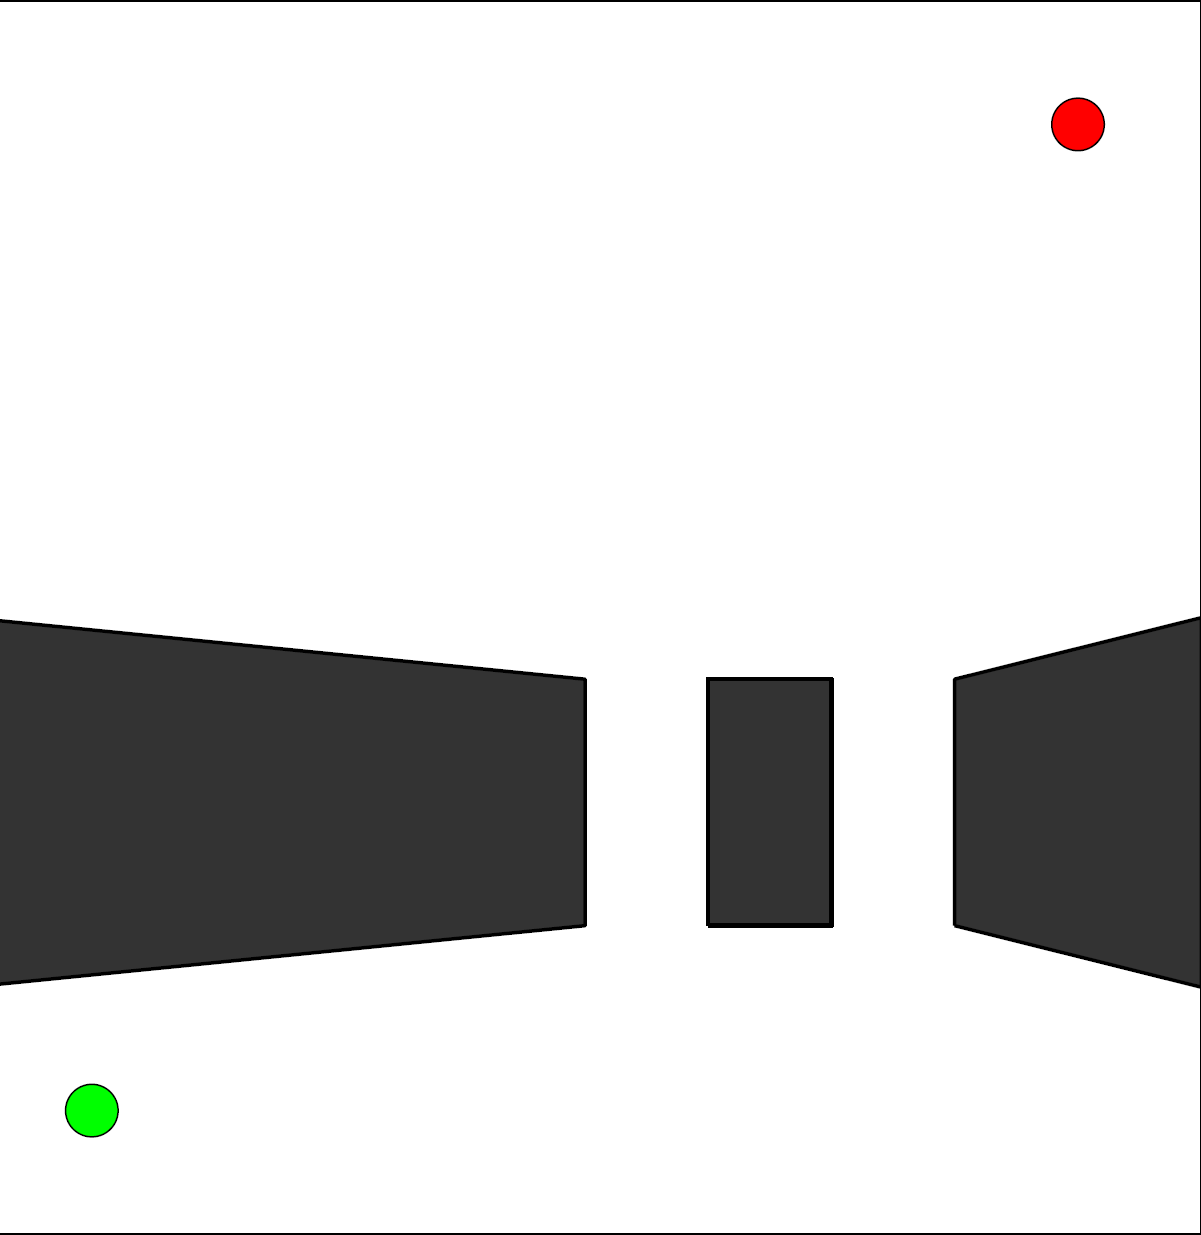
\includegraphics[width=0.48\linewidth]{4-a}}
	\hfill
	\subfigure[]{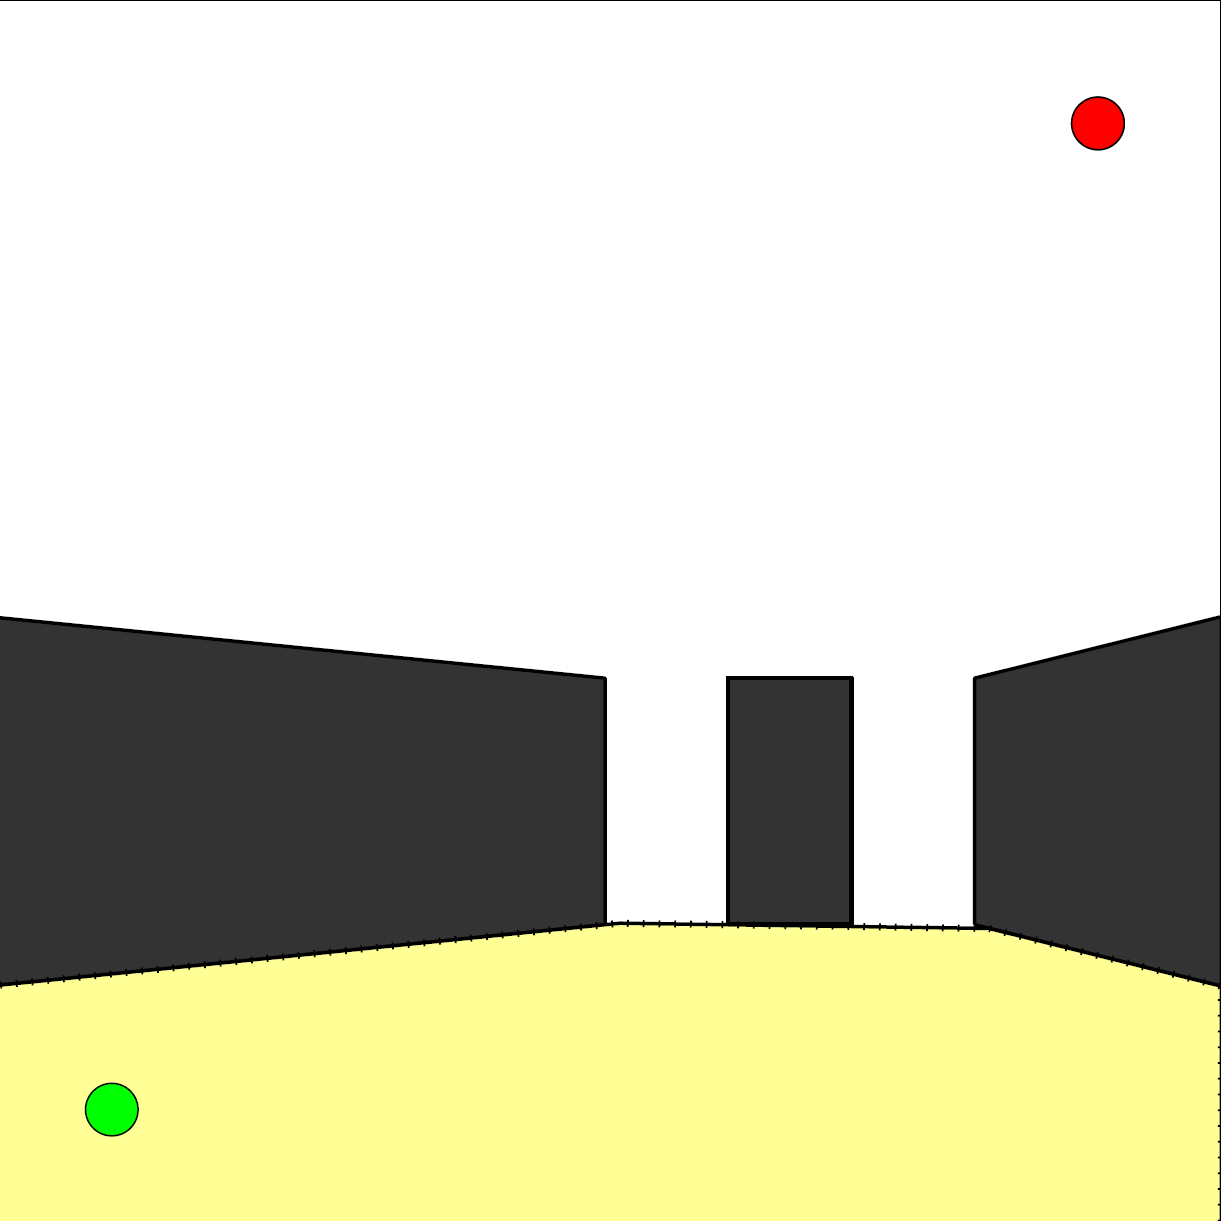
\includegraphics[width=0.48\linewidth]{4-b}}
	\hfill
	\subfigure[]{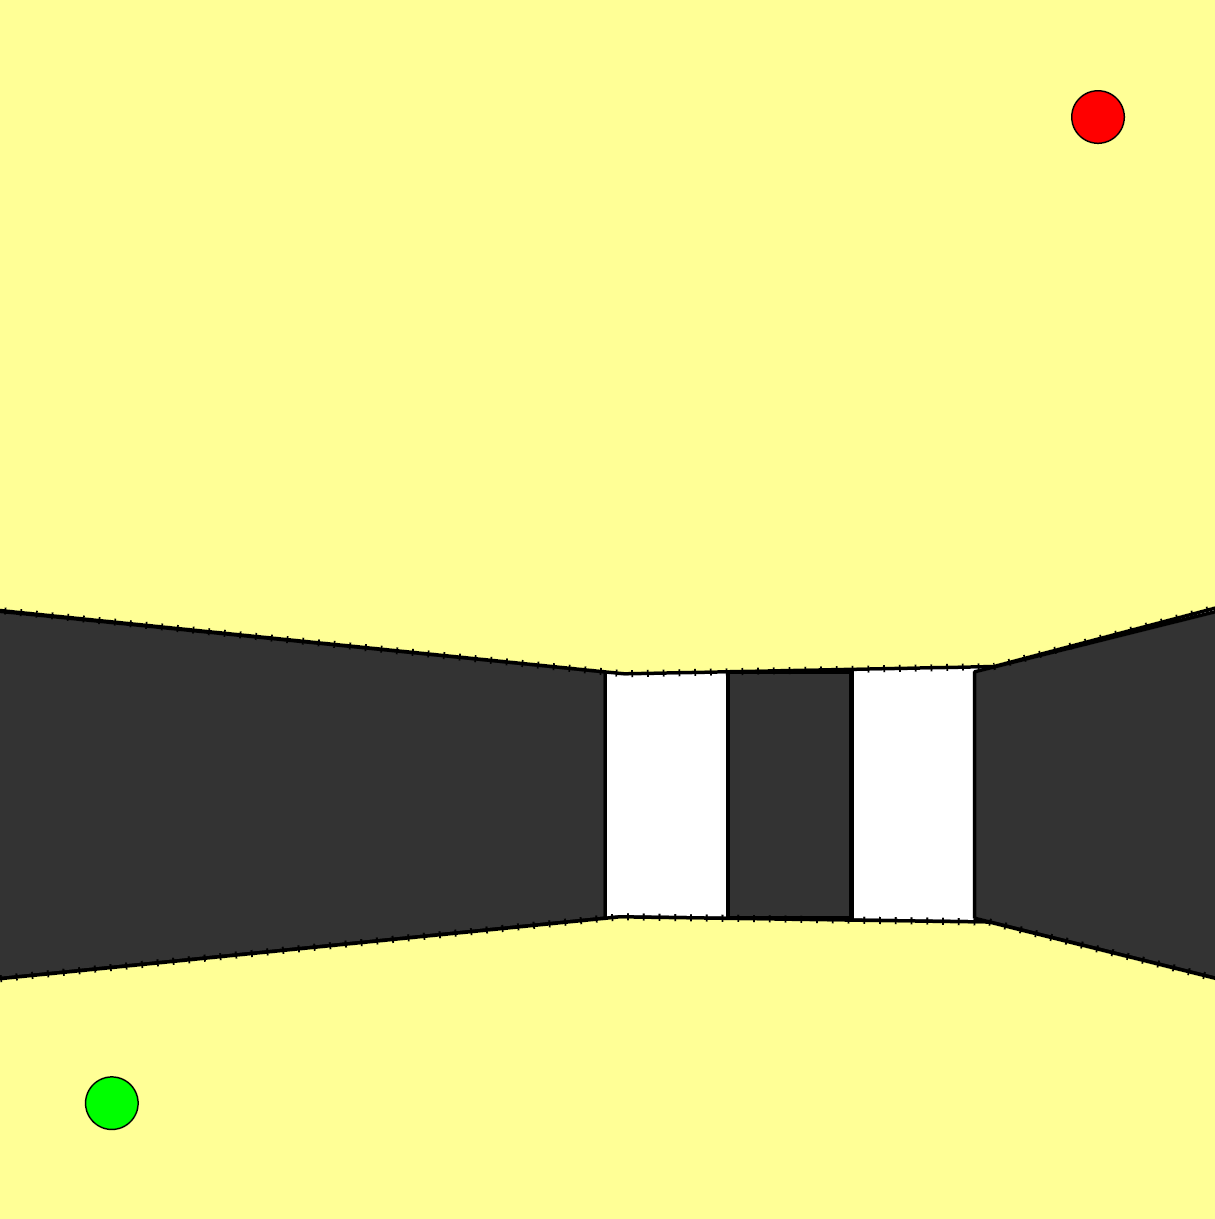
\includegraphics[width=0.48\linewidth]{4-c}}
	\hfill
	\subfigure[]{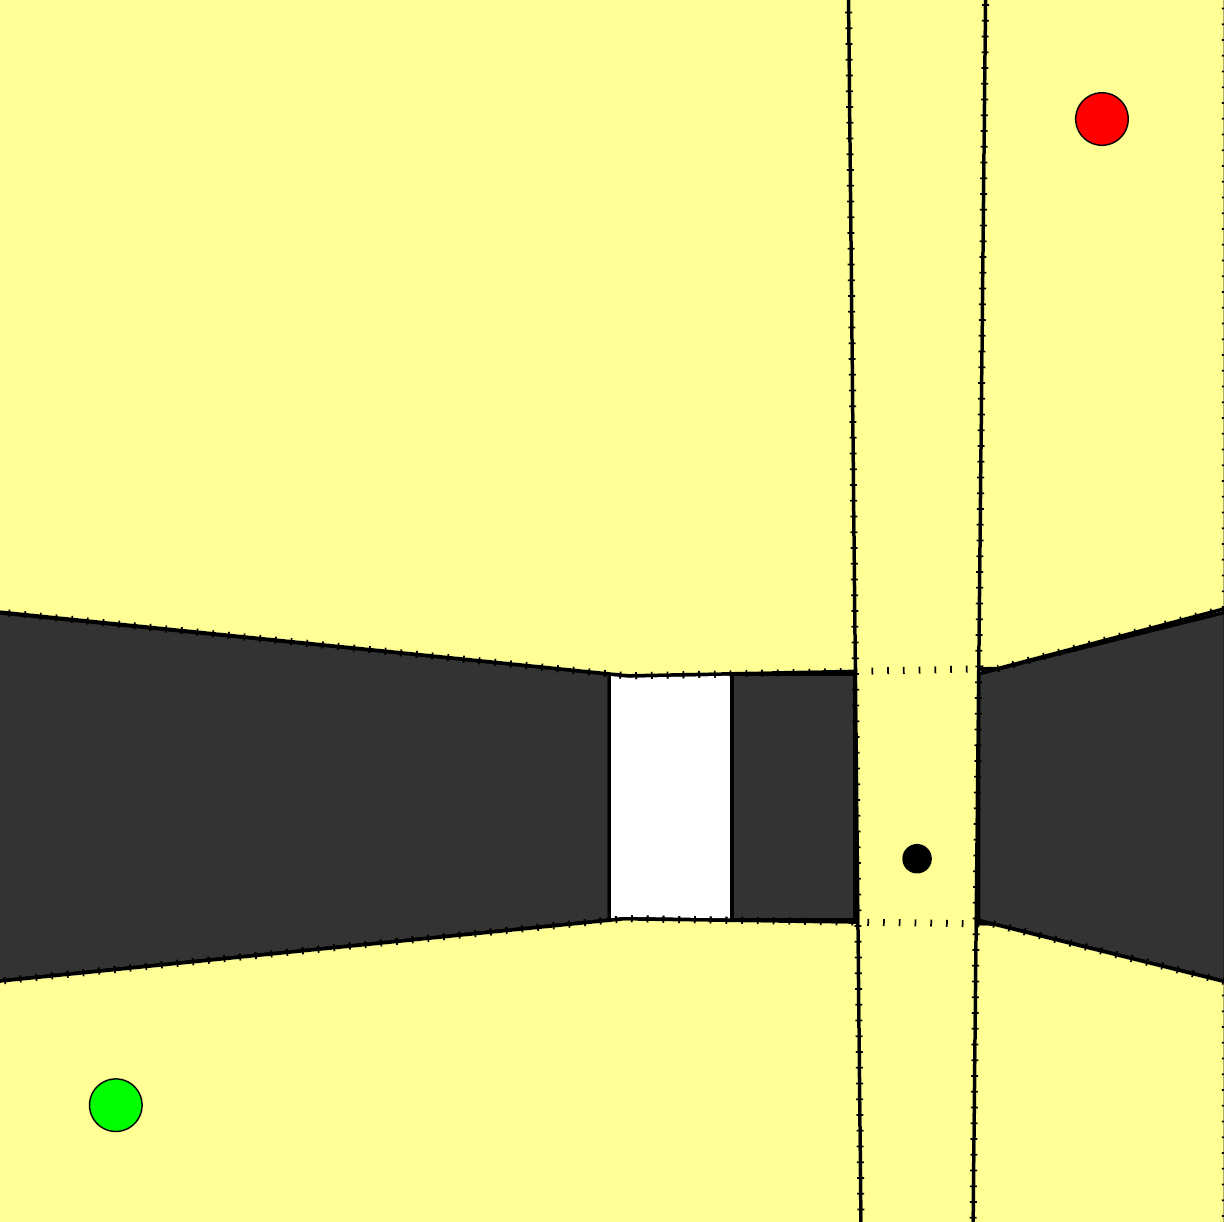
\includegraphics[width=0.48\linewidth]{4-d}}
	\hfill
	\caption{\label{fig: figs-4a}Solving a simple environment with IRIS regions. A random environment is constructed with obstacles and a start and goal pose (a), then generate IRIS regions around the start (b) and goal (c). Next, a point is identified far from the existing set of obstacles and IRIS regions and a new region is generated from the seed point there (d)}
\end{figure}
\begin{figure}[t]
	\hfill
	\subfigure[]{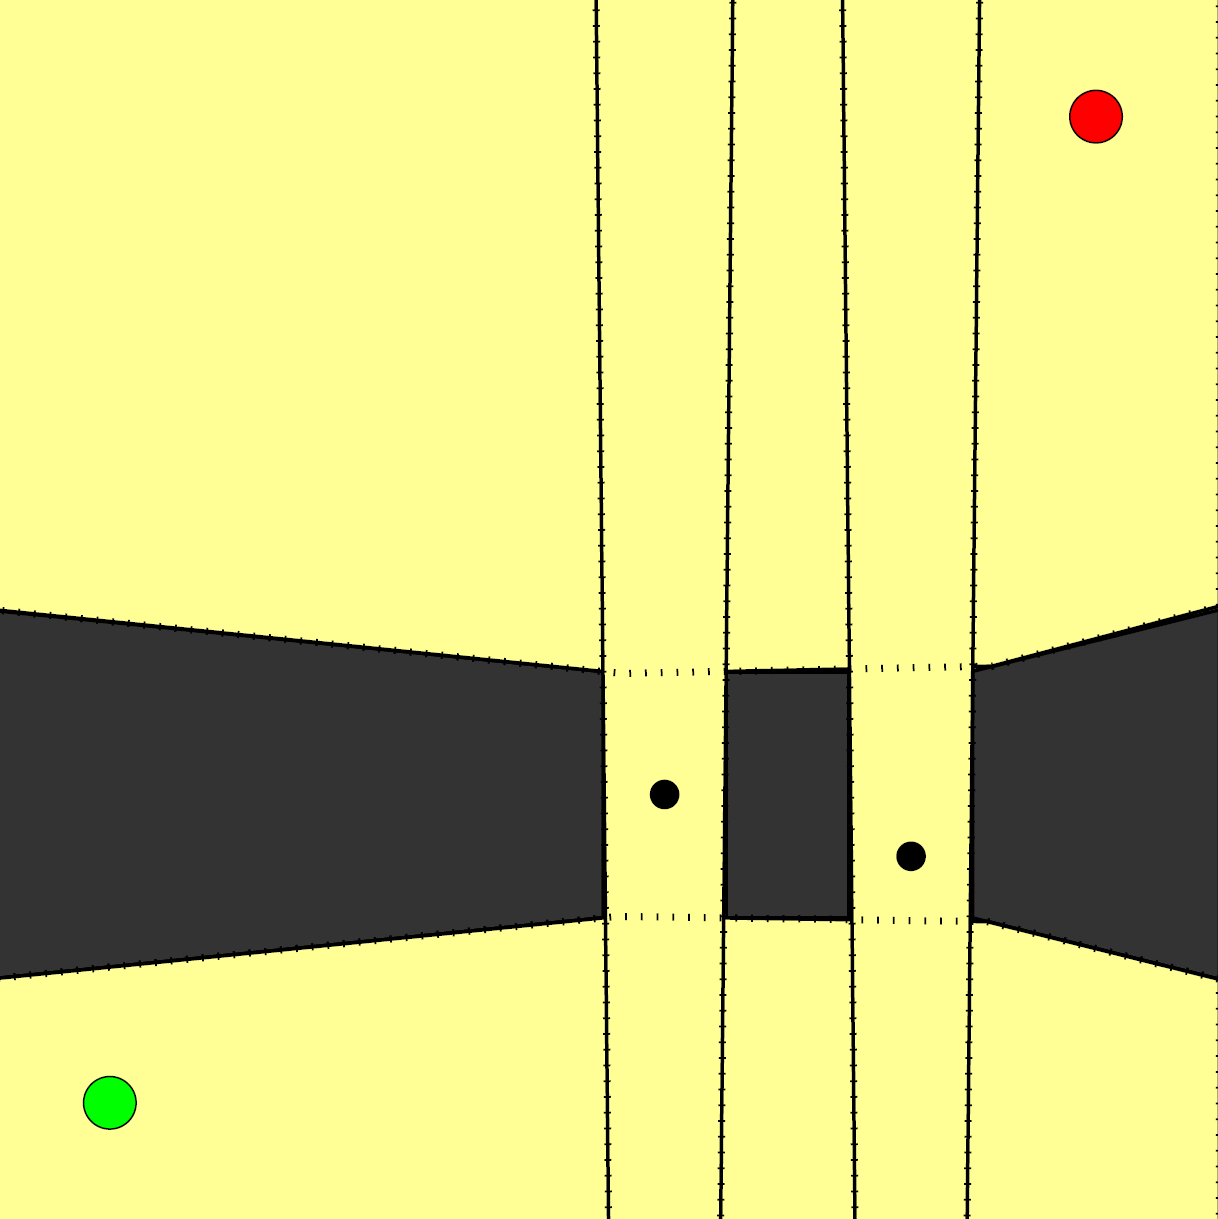
\includegraphics[width=0.48\linewidth]{4-e}}
	\hfill
	\subfigure[]{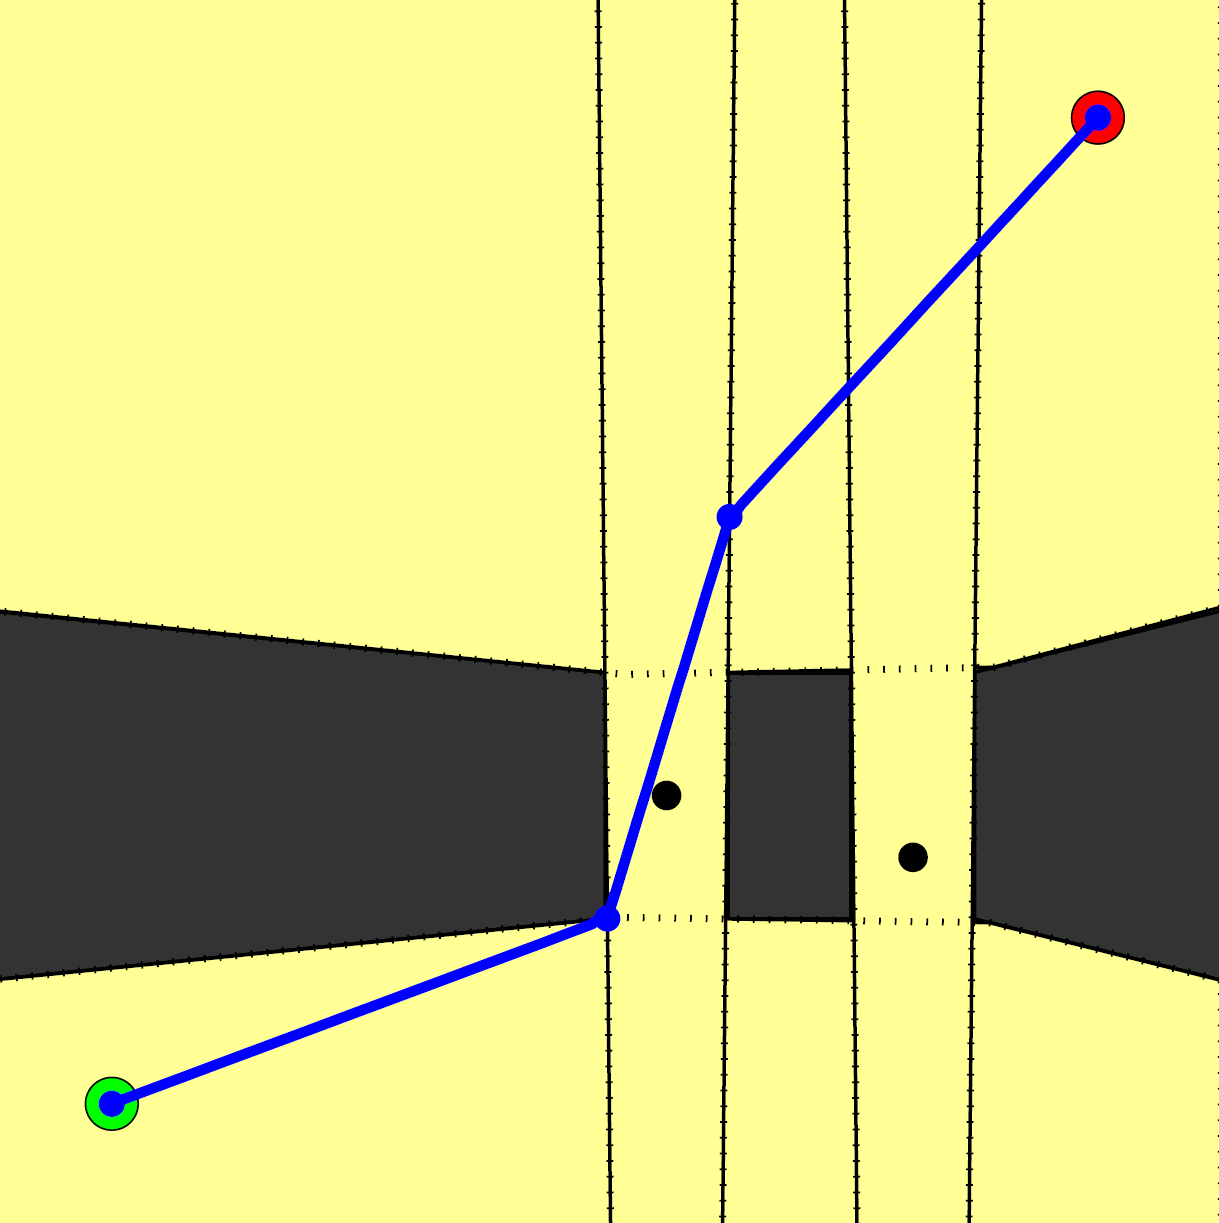
\includegraphics[width=0.48\linewidth]{4-f}}
	\hfill
	\subfigure[]{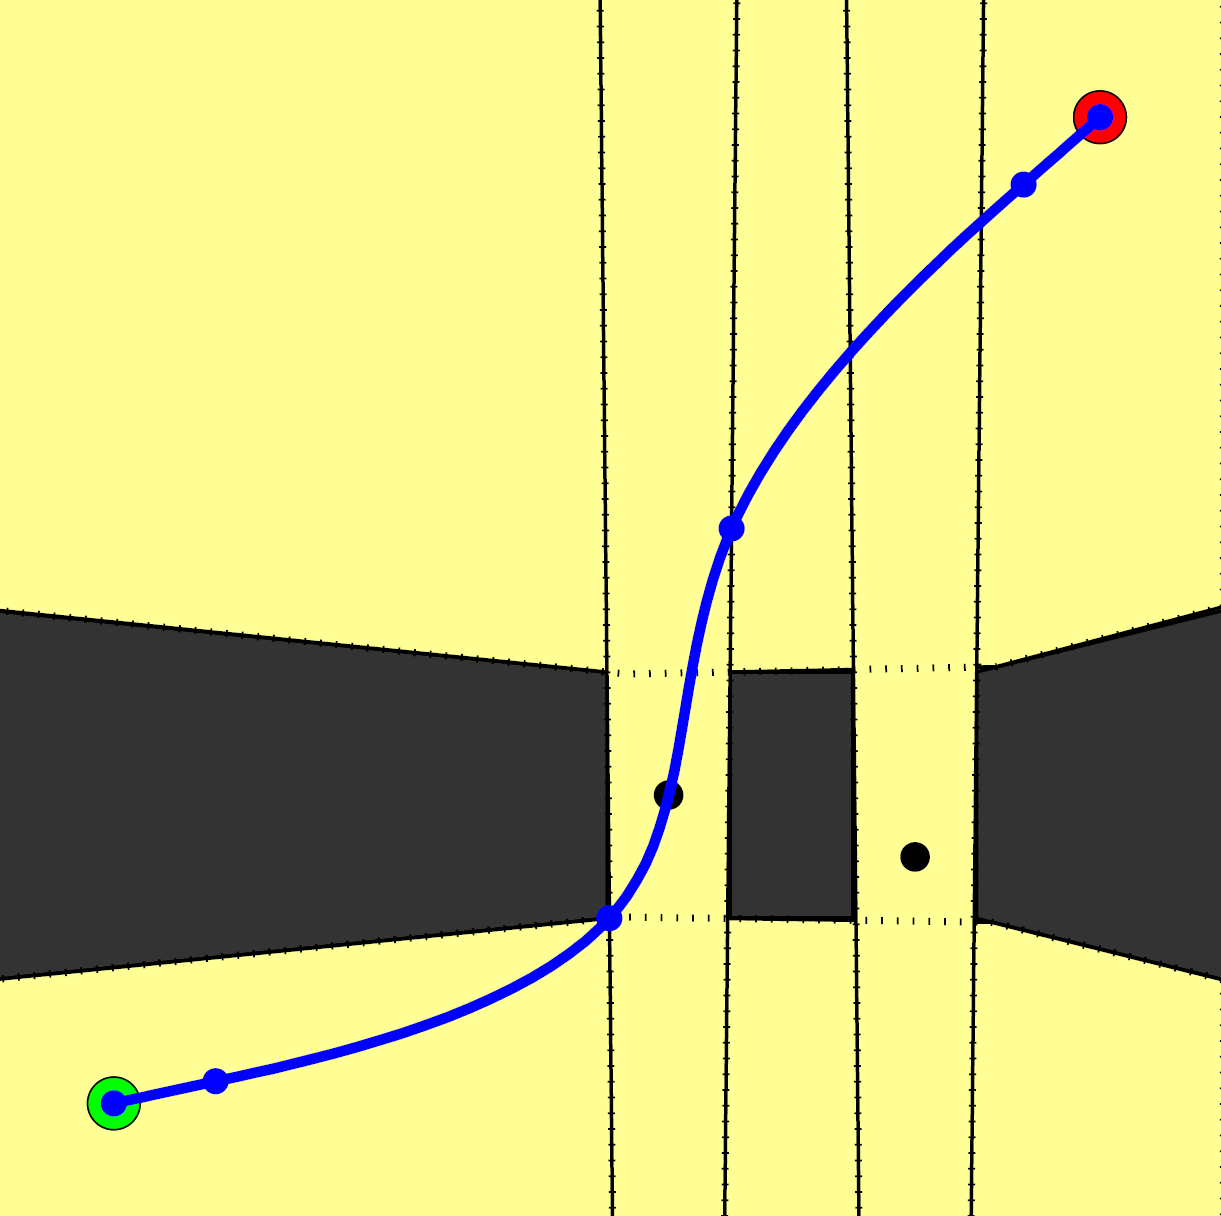
\includegraphics[width=0.48\linewidth]{4-g}}
	\hfill
	\subfigure[]{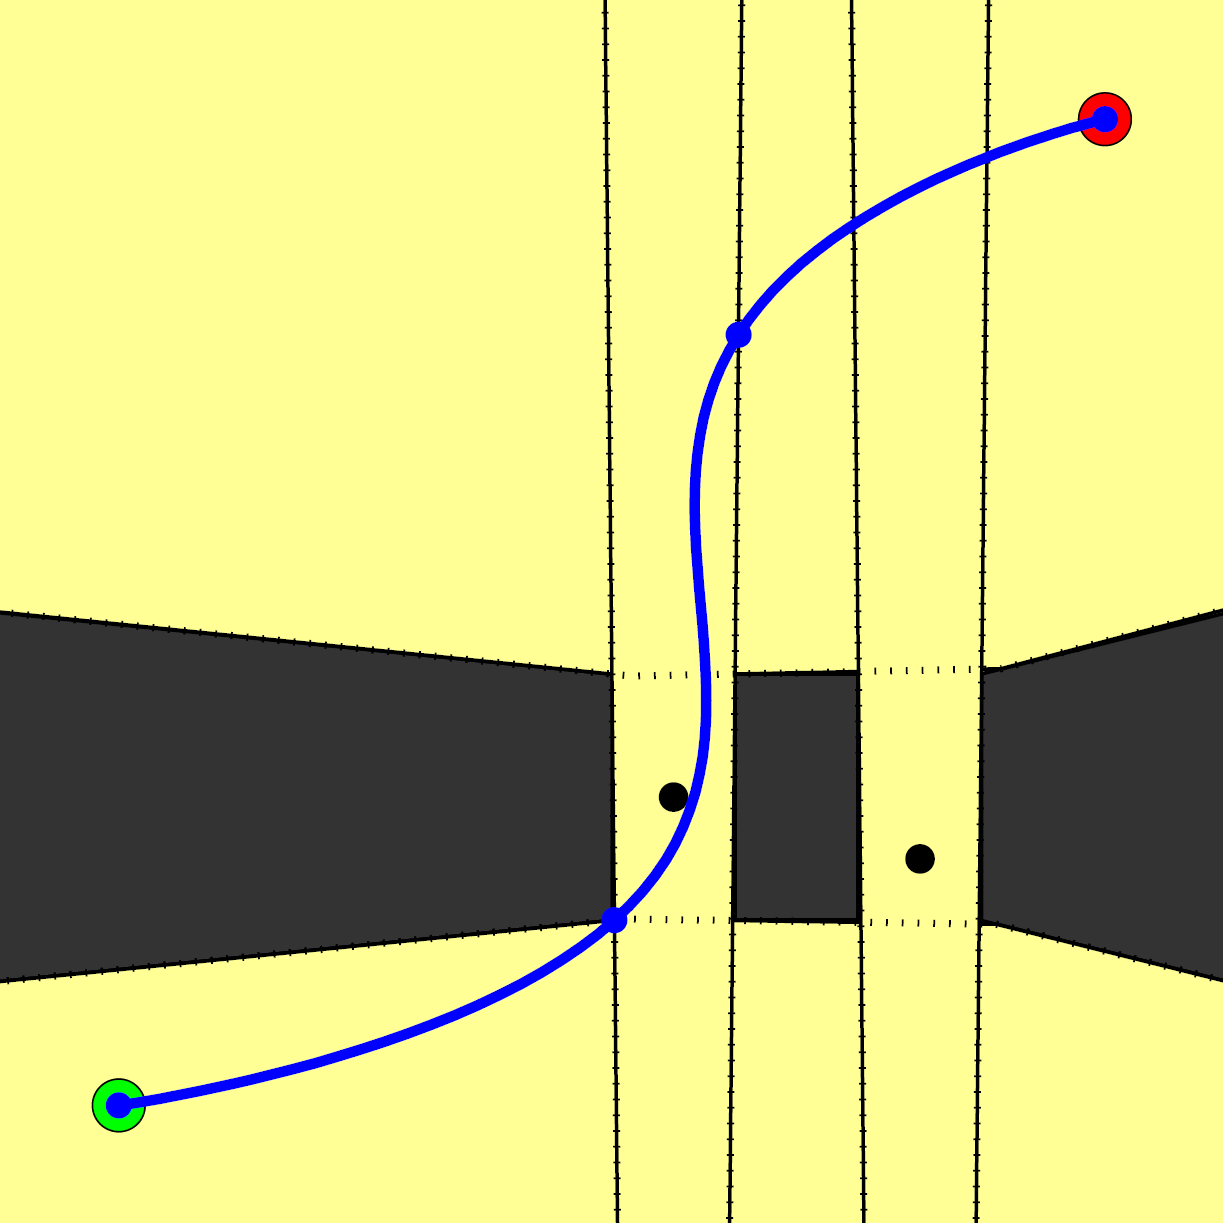
\includegraphics[width=0.48\linewidth]{4-h}}
	\hfill
	
	
	\caption{\label{fig: figs-4b}The above process through which we obtained (d) is repeated until we have 4 regions (e). Finally, we solve for trajectories of $1^{st}$-degree polynomials minimizing squared velocity in 0.1s (f), $3^{rd}$-degree polynomials minimizing squared jerk in 0.3s (g), and
		$5^{th}$-degree polynomials minimizing squared snap in 1.0s (h). All trajectories lie entirely within the convex regions shown.}
\end{figure}



\section{Handling Lower-Degree Trajectories}
Even if the mixed-integer optimization is done over the numerically easier degree $3$ polynomials, we can post-process the resulting trajectories in order to successfully use the differential flatness of the system to derive the full state and input. A piecewise degree-$3$ trajectory has a piecewise constant $3^{rd}$ derivative. It thus has delta functions for its $4^{th}$ derivative, which Mellinger relates directly to the rotor thrusts of the
UAV~\cite{mellinger2011minimum}. Since this is clearly undesirable, according the proposed approach we proceeded as follows: First, we ran the MISOCP to optimize our degree-$3$ polynomials and assign them to convex safe regions. Next, we fixed the resulting assignment of trajectories to safe regions and then re-ran the optimization for polynomials of degree
$5$ or higher while minimizing the squared norm of the snap. Since all of the integer variables are fixed, we no longer have a mixed-integer problem but instead a single semidefinite program, which can be solved very efficiently. 

\section{Complete Formulation}

Our optimization problem can be written as follows for a
trajectory of $N$ piecewise $3^{rd}$-degree polynomials:

	
\begin{equation}  \label{eq:eq20_deits}
\min_{P,H,\sigma} \quad  \sum_{j=1}^{N} \begin{Vmatrix}\frac{\mathrm{d}^3 }{\mathrm{d} t^3}
P_{j}(t) 
\end{Vmatrix}
\end{equation}subject to:


\[
\begin{array}{@{}l@{}} 
P_{1}(0) = {x_{0}}, \quad {P_{N}}(1) = {x_{f}}, \quad  {P_{j}}(1) = {P_{j+1}}(0) \\

{\dot{P_1}}(0) = {\dot{x_0}}, \quad {\dot{P_N}}(1) = c{\dot{x_f}}, \quad {\dot{P_j}}(1) = {\dot{P}_{j+1}}(0) \\

{\ddot{P_1}}(0) = {\ddot{x_0}}, \quad {\ddot{P_N}}(1) = {\ddot{x_f}}, \quad {\ddot{P_j}}(1) = {\ddot{P}_{j+1}}(0)

\end{array}
\]

\begin{equation}
	\forall j \in \begin{Bmatrix}1,
	&.  &.  &. & ,N 
	\end{Bmatrix}
\end{equation}

where $\sigma_{l,j,1}(t), \sigma_{l,j,2}(t) $ are sums of squares

	\[
	\begin{array}{@{}l@{}} 
	{H_{r,j}} \implies\\ \quad {b_{r,m}} - {A_{r,m}^{T}}{p_{j}}(t) = t{\sigma_{j,m,1}}(t) + (T_j - t){\sigma_{j,m,2}}(t)  \\ 
	
	\end{array}
	\]


\[
\begin{array}{@{}l@{}} 
\sum_{r=1}^{R}{H_{r,j}} = 1 \quad \forall j \in {1, ..., N}  \\ 
\end{array}
\]
	\begin{equation}  \label{eq:eq24_deits}
 {H_{r,j}} \in {0,1}
	\end{equation}
	
	where ${x_{0}}$ , $\dot{x_0}$ , $\ddot{x_0}$ are the initial position, velocity, and 	acceleration of the vehicle and ${x_{f}}$ , $\dot{x_f}$ , $\ddot{x_f}$ are the final values. All of the above conditions are linear constraints on the coefficients $C$ and $\beta$ and the matrix $H$, except the condition that $\sigma_1$ and $\sigma_2$ are sums of squares, which is a rotated second-order cone constraint.	 
